\section{File-level redundant ratio}
\label{sec:dedup}

\subsection{Overview of redundant file overhead}

\begin{figure}
	\centering
	%\includegraphics [width=0.45\textwidth]{plots/exp-total-stev-erase.eps}
	\subfigure[File-level dedup model]{\label{fig:over-dup-overhead-cnt}
		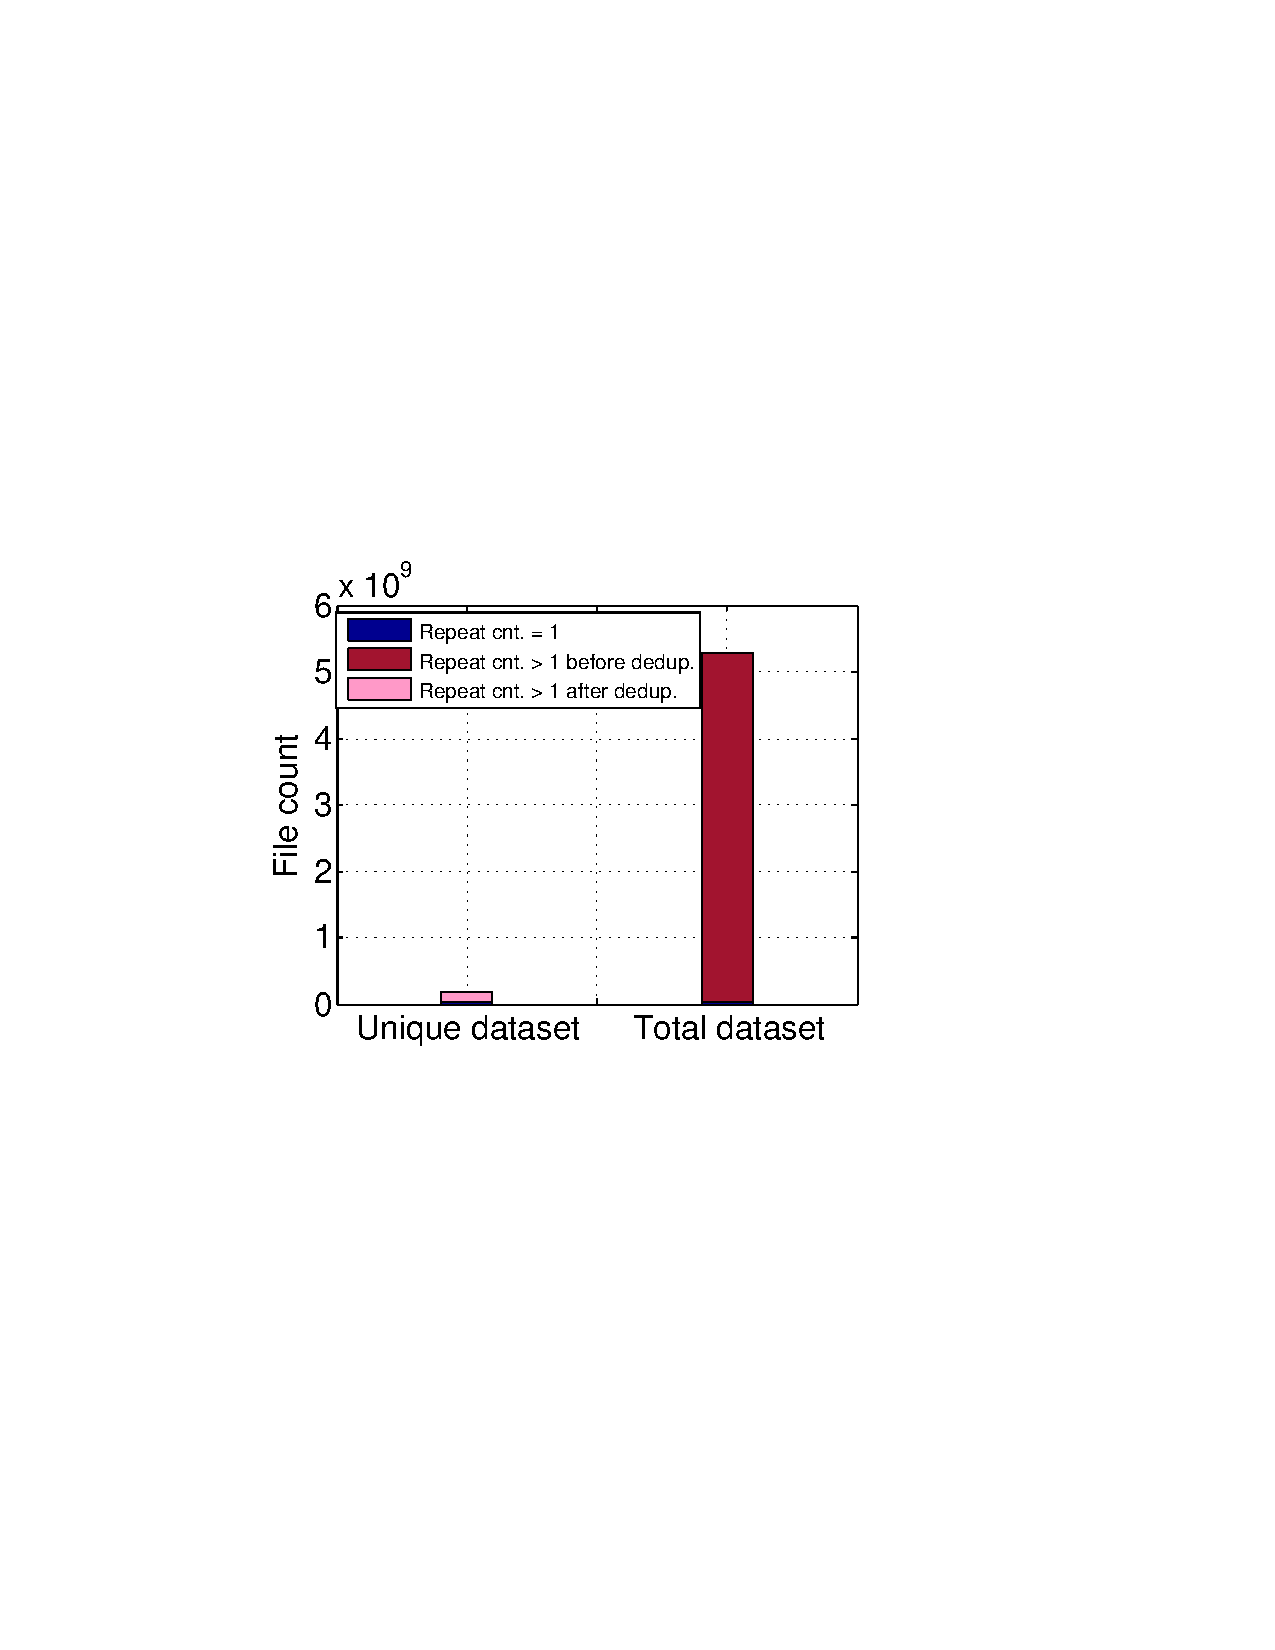
\includegraphics [width=0.21\textwidth]{graphs/dup-ratio-cnt.pdf}
	}
	\subfigure[Similar layer dedup]{\label{fig:over-dup-overhead-cap}
		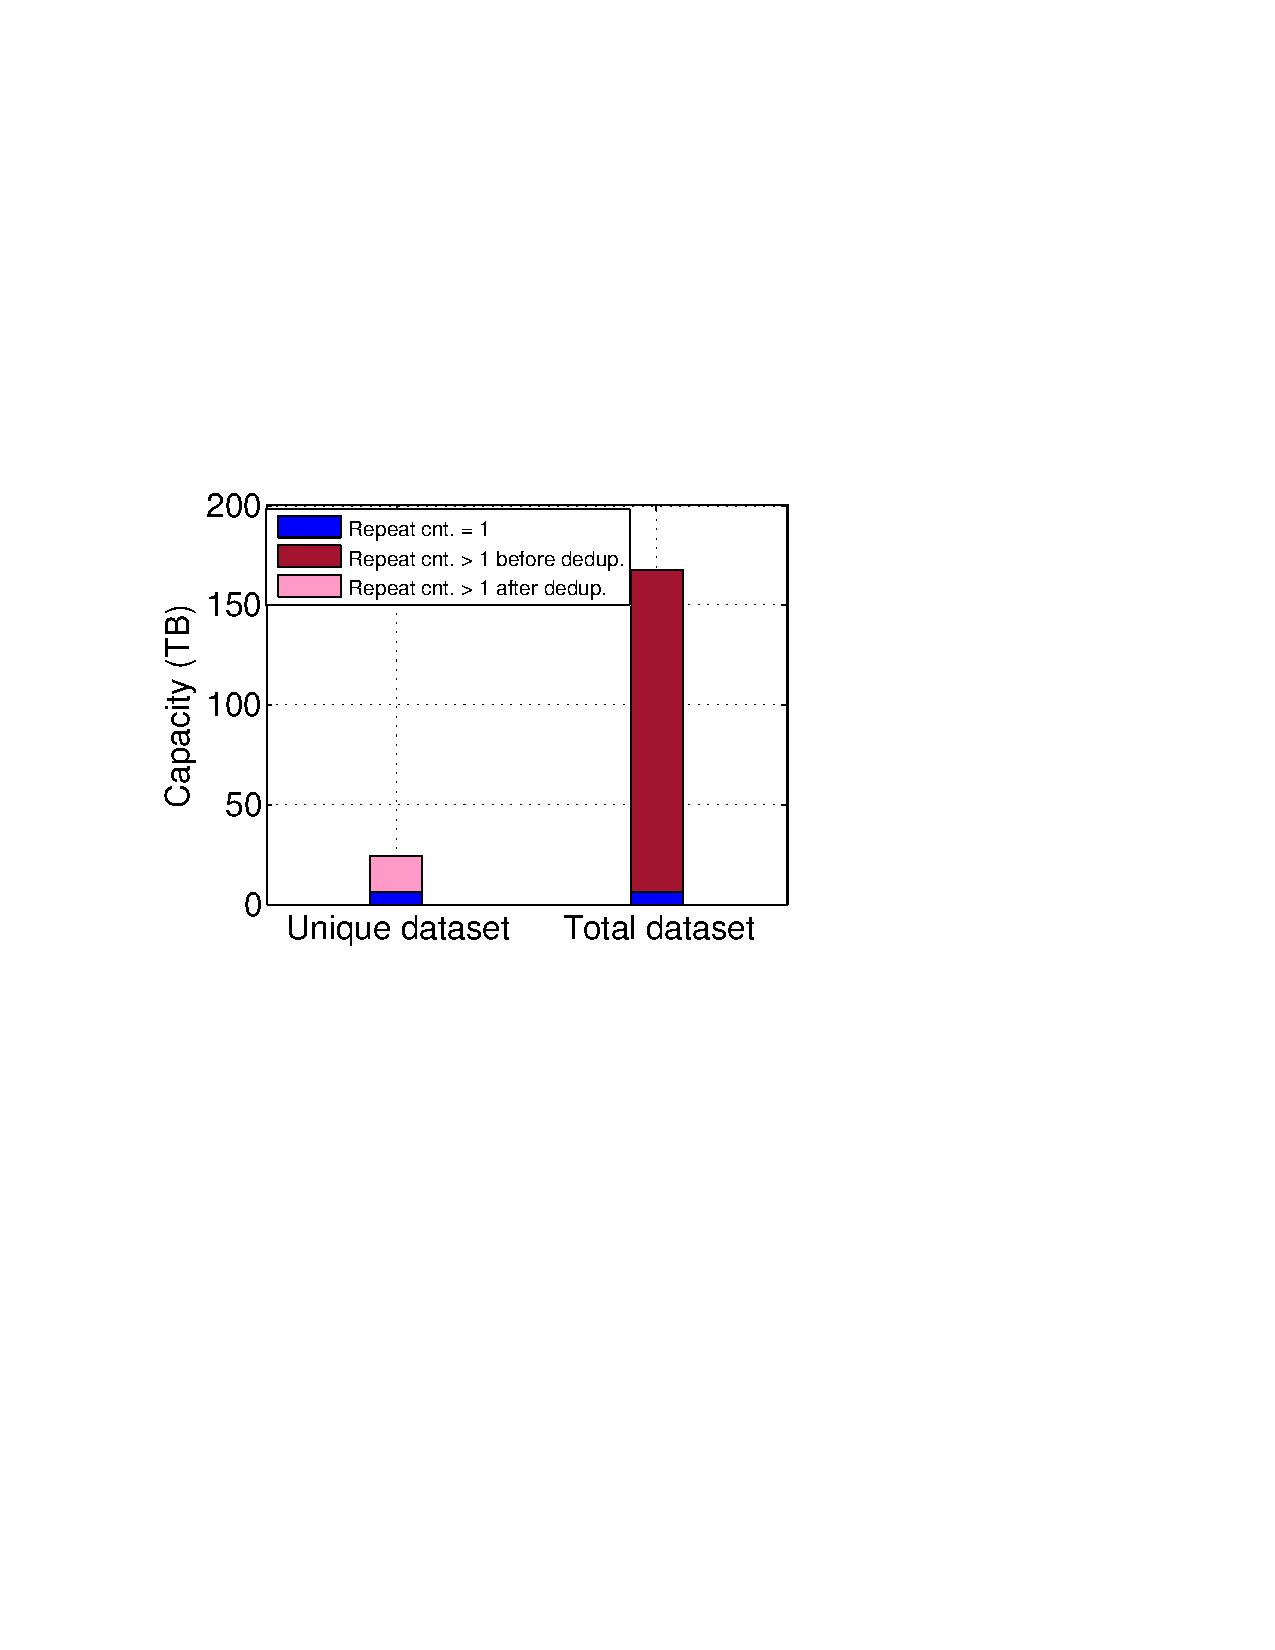
\includegraphics [width=0.225\textwidth]{graphs/dup-ratio-cap.pdf}
	}
	\caption{Redundant storage overhead.}
	\label{fig:over-dup-overhead}
\end{figure}

\begin{table} 
	\centering 
	\scriptsize  
	%\begin{minipage}{.5\linewidth}
	\caption{Redundant ratio in terms of file count and capacity} \label{tbl:overall-redundant_ratio} 
	\begin{tabular}{|l|l|l|}%p{0.14\textwidth} 
		\hline  
		       & File count & Capacity \\
		\hline
		Repeat cnt = 1 & 0.58\% & 10.87\%\\
		\hline
		Repeat cnt $>$ 1 after dedup & 2.59\% & 3.44\%\\
		\hline
		Repeat cnt $>$ 1 before dedup  & 99.42\%  & 89.13\%\\
		\hline
		Unique dataset (Uncompressed) & 3.17\% (167,251,437)  &  14.31\% (23.92 TB) \\
		\hline 
		Total dataset (Uncompressed) & 5,278,465,130 & 167.20 TB \\
		\hline 	
		%\hline 
	\end{tabular} 
\end{table} 

\subsection{Redundant ratio for layers}

\begin{eqnarray}
r_{intra\_dedup.} = \frac{S_{uncompress.} - S_{dropdup.}}{S_{uncompress.}} \\
r_{inter\_dedup.} = \frac{S_{uncompress.} - S_{shares}}{S_{uncompress.}}
\end{eqnarray}

\paragraph{Intra-layer redundant ratio} Intra-layer redundant ratio is shown in Figure~\ref{fig:layer-dedup_cdf_and_hist_layer}.

\begin{figure}
	\centering
	\subfigure[CDF of intra/inter-layer redundant ratio in terms of file count/capacity]{\label{fig:layer-dedup-cdf}
		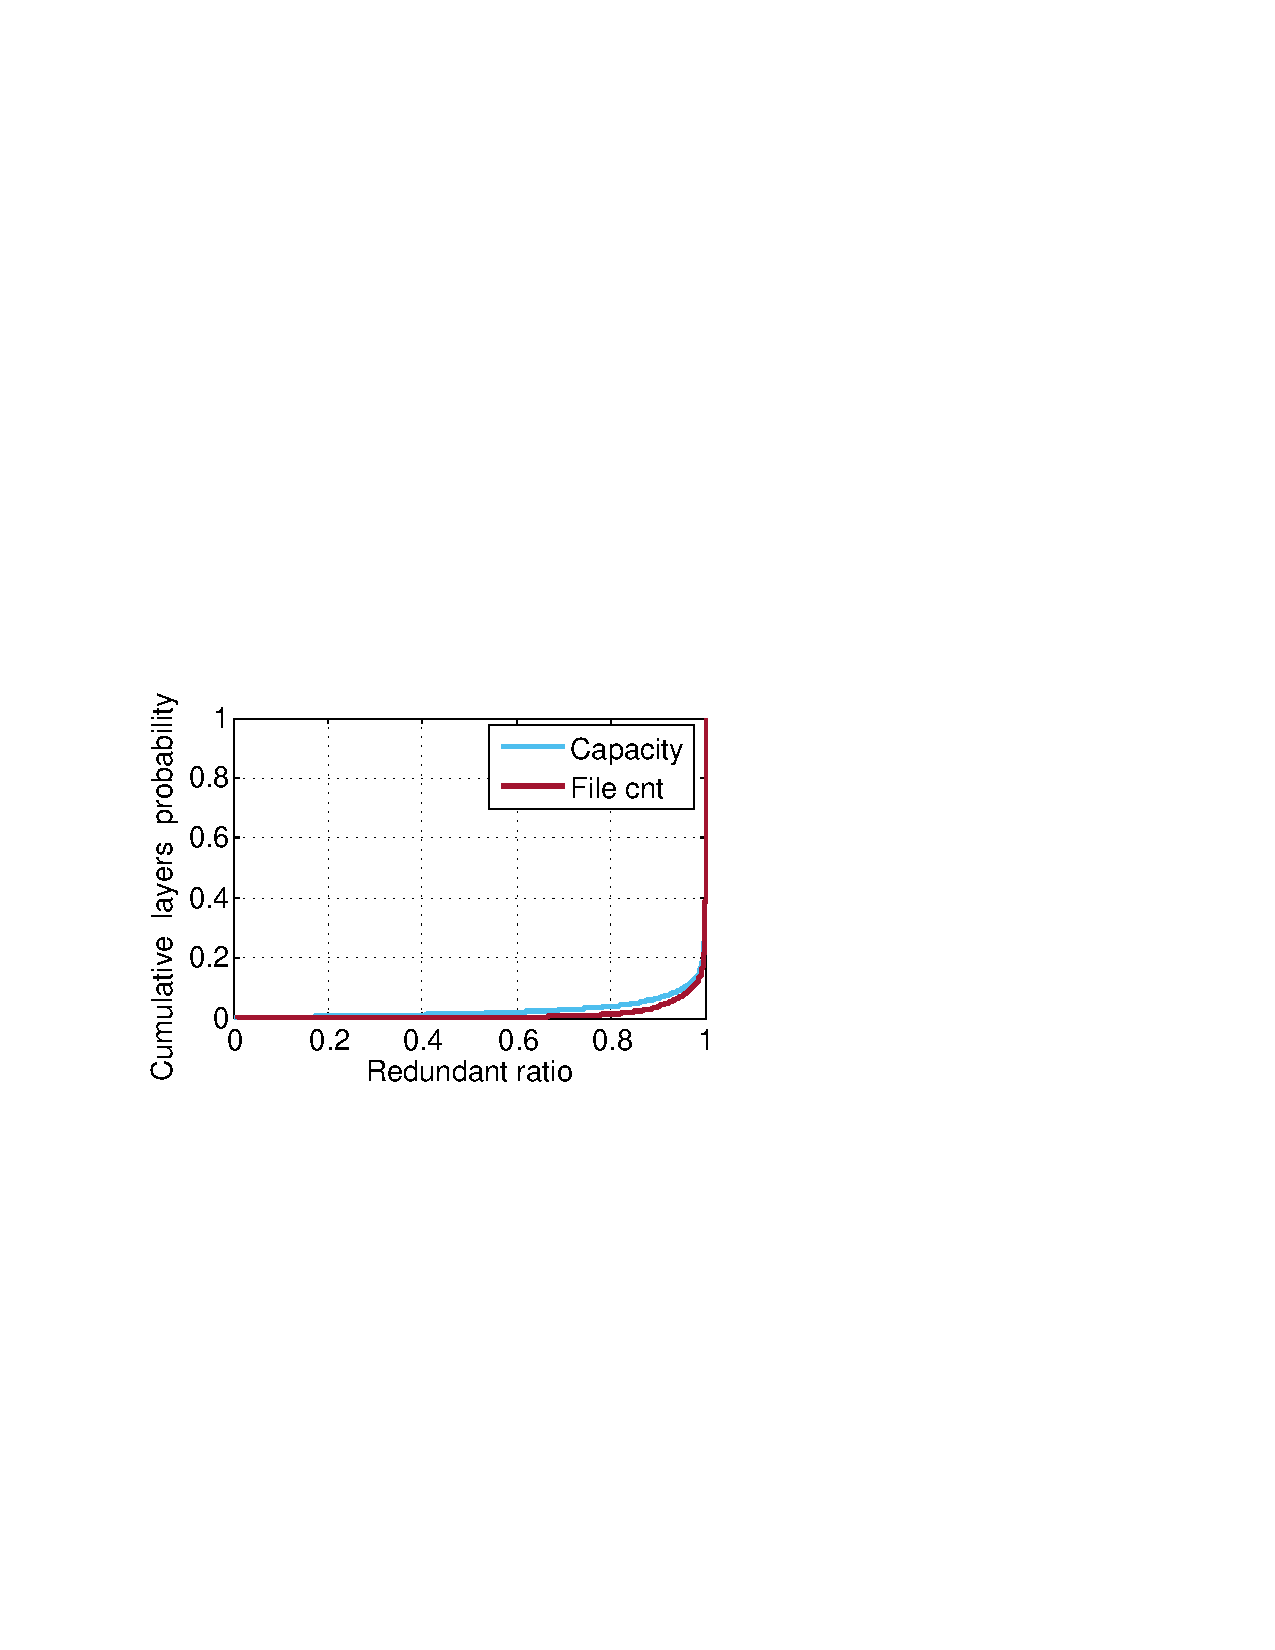
\includegraphics [width=0.4\textwidth]{graphs/layer-dup-ratio-cdf}
	}
	\subfigure[Histogram of intra/inter-layer redundant ratio in terms of file count/capacity]{\label{fig:layer-dedup_hist}
		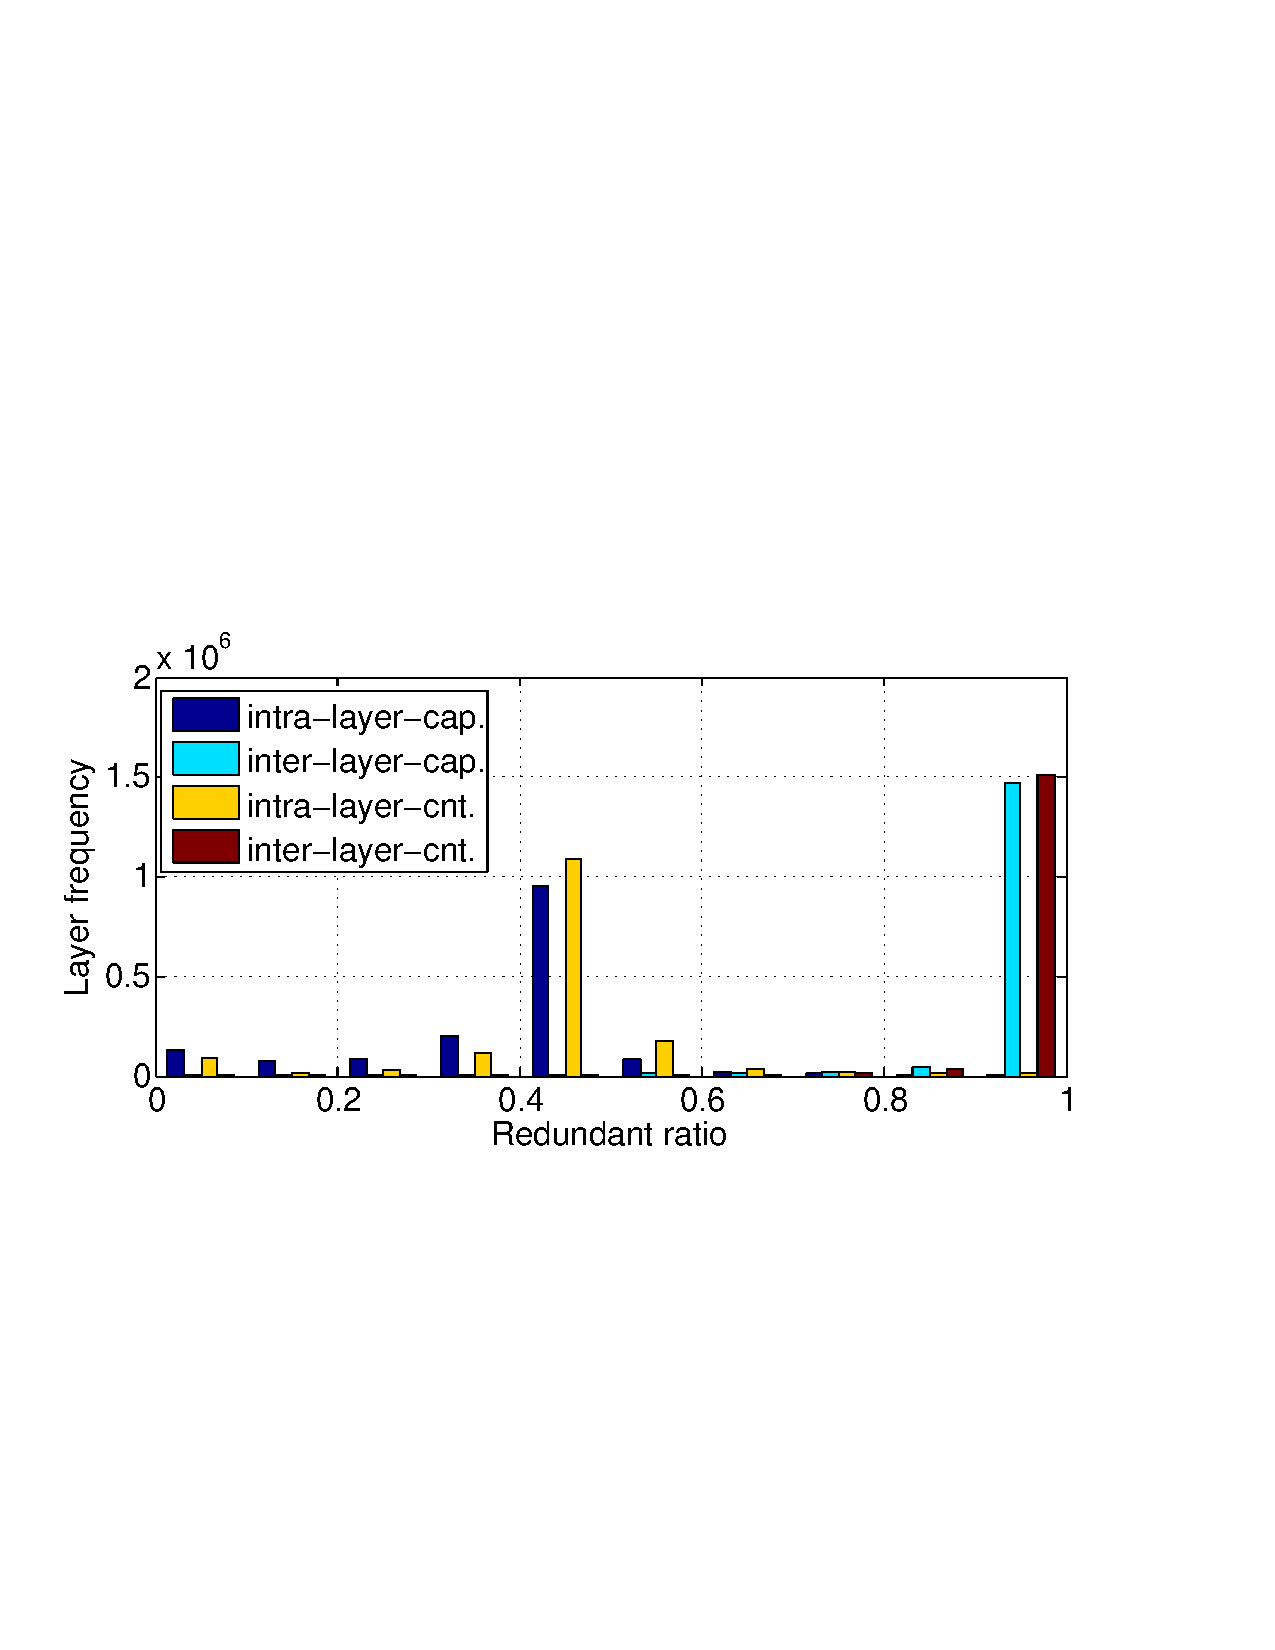
\includegraphics [width=0.4\textwidth]{graphs/layer-dup-ratio-pdf}
	}
	\caption{Layer redundant ratio}
	\label{fig:layer-dedup-ratio}
\end{figure}

\paragraph{Inter-layer redundant ratio} Inter-layer redundant ratio is shown in Figure~\ref{fig:layer-dedup_cdf_and_hist_layer}

\subsection{Redundant ratio for images}

\begin{figure}
	\centering
	\subfigure[CDF of intra/inter-image redundant ratio in terms of file count/capacity]{\label{fig:image-dedup_cdf}
		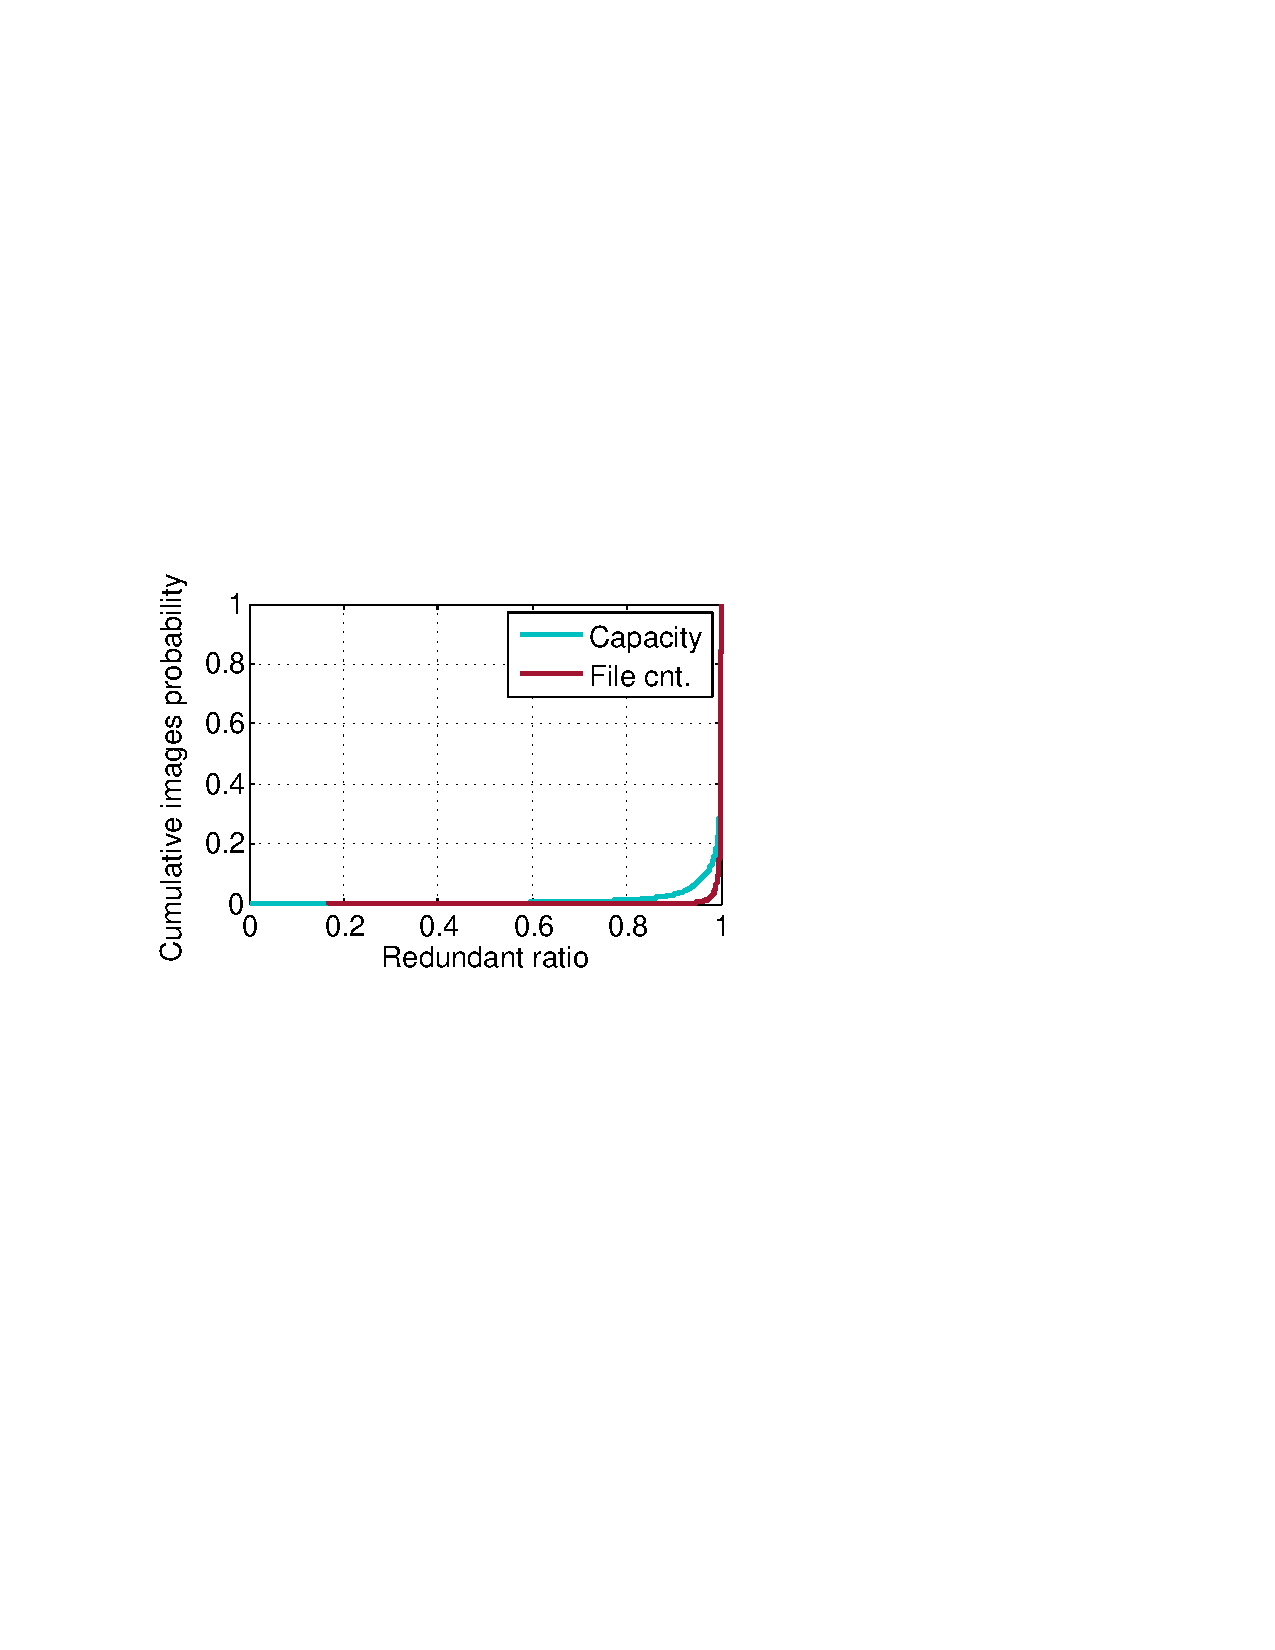
\includegraphics [width=0.4\textwidth]{graphs/image-dup-ratio-pdf}
	}
	\subfigure[Histogram of intra/inter-image redundant ratio in terms of file count/capacity]{\label{fig:image-dedup_hist}
		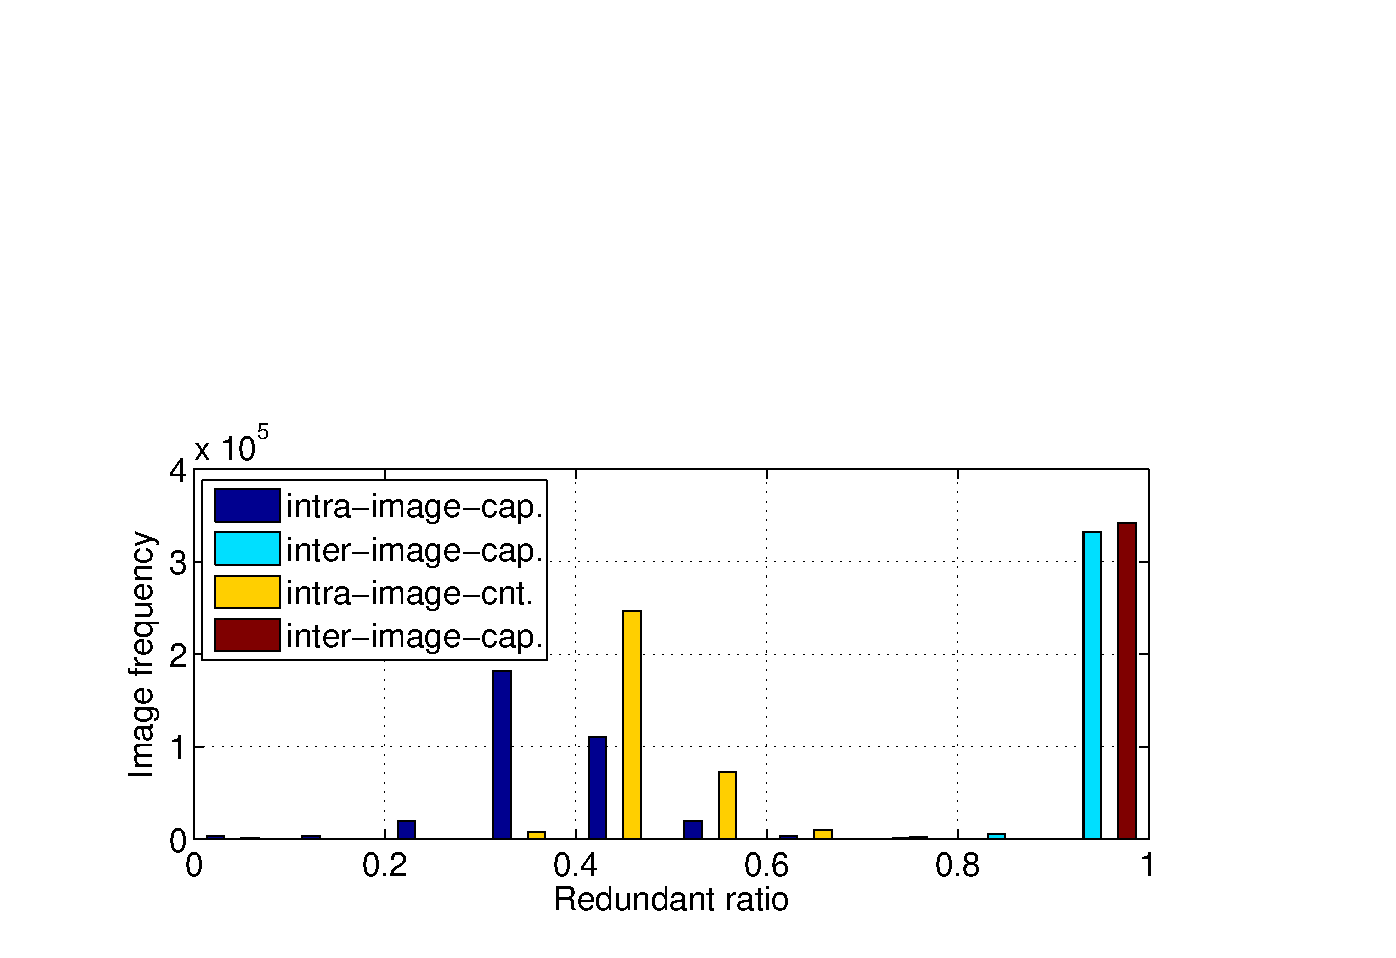
\includegraphics [width=0.4\textwidth]{graphs/image-dup-ratio-cdf}
	}
	\caption{Image redundant ratio}
	\label{fig:image-dedup-ratio}
\end{figure}
\paragraph{Intra-image redundant ratio} Intra-image redundant ratio is shown in Figure~\ref{fig:image-dedup_cdf_and_hist_layer}

\paragraph{Inter-image redundant ratio} Inter-image redundant ratio is shown in Figure~\ref{fig:image-dedup_cdf_and_hist_layer}


%=======================================
%|             OLD VERSION              |
%=======================================
%\subsubsection{Overview of redundant ratio for layers}
%\begin{table} 
%	\centering 
%	\scriptsize  
%	%\begin{minipage}{.5\linewidth}
%	\caption{Intra-layer redundant ratio for layers in terms of file count and capacity} \label{tbl:intra_dup_ratio_layers} 
%	\begin{tabular}{|l|l|l|}%p{0.14\textwidth} 
%		\hline 
%		% after \\: \hline or \cline{col1-col2} \cline{col3-col4} ... 
%		% after \\: \hline or \cline{col1-col2} \cline{col3-col4} ... 
%		& File count & Capacity \\
%		\hline
%		Avg. & 49.78\% & 40.09\%\\
%		\hline
%		Median & - & - \\
%		\hline
%		Max. & 99.99\% & 99.99\%\\
%		\hline
%		Min.  & 0.00\%  & 0.00\%\\
%		\hline
%		Stdev.  &  2.14\% & 17.18\%\\
%		\hline
%		Layer dataset after intra.-dedup (Uncompressed) & -  & -\\
%		\hline 
%		Total layer dataset (Uncompressed) &  -	& -\\
%		\hline 
%		%\hline 
%	\end{tabular} 
%\end{table}

%\begin{table} 
%	\centering 
%	\scriptsize  
%	%\begin{minipage}{.5\linewidth}
%	\caption{Inter-layer redundant ratio for layers in terms of file count and capacity} \label{tbl:inter_dup_ratio_layers} 
%	\begin{tabular}{|l|l|l|}%p{0.14\textwidth} 
%		\hline 
%		% after \\: \hline or \cline{col1-col2} \cline{col3-col4} ... 
%		% after \\: \hline or \cline{col1-col2} \cline{col3-col4} ... 
%		& File count & Capacity \\
%		\hline
%		Avg. & 98.75\% & 97.33\%\\
%		\hline
%		Median & - & - \\
%		\hline
%		Max. & 1 & 1\\
%		\hline
%		Min.  & 0.87\%  & $<$ 0.00\%\\
%		\hline
%		Stdev.  &  4.70\% & 10.49\\
%		\hline
%		Layer dataset after inter.-dedup (Uncompressed) & -  & -\\
%		\hline 
%		Total layer dataset (Uncompressed) &  -	& -\\
%		\hline
%	\end{tabular} 
%\end{table}

%\subsubsection{Redundant ratio distribution}

%\paragraph{Cumulative distribution for intra-layer redundant ratio and inter-layer redundant ratio in terms of file count and storage capacity}



%\paragraph{Intra-layer redundant ratio by layer size in terms of file count and storage capacity}

%\begin{figure}
%	\centering
%	\includegraphics[width=0.5\textwidth]{graphs/inter-dedup-by-size.eps}
%	\caption{Intra-layer redundant ratio by layer size.
%	}
%	\label{fig_redundant_overhead}
%\end{figure}

%\subsubsection{Inter-layer redundant overhead}

%\paragraph{Histogram of intra-layer redundant ratio and inter-layer redundant ratio in terms of file count and storage capacity}

%\paragraph{Inter-layer redundant ratio by layer size in terms of file count and storage capacity}

%\subsubsection{Overview of redundant ratio for images}

%\begin{table} 
%	\centering 
%	\scriptsize  
%	%\begin{minipage}{.5\linewidth}
%	\caption{Inter-layer redundant ratio for images in terms of file count and capacity} \label{tbl:intra_dup_ratio_images} 
%	\begin{tabular}{|l|l|l|}%p{0.14\textwidth} 
%		\hline 
%		% after \\: \hline or \cline{col1-col2} \cline{col3-col4} ... 
%		% after \\: \hline or \cline{col1-col2} \cline{col3-col4} ... 
%		& File count & Capacity \\
%		\hline
%		Avg. & 98.75\% & 97.33\%\\
%		\hline
%		Median & - & - \\
%		\hline
%		Max. & 1 & 1\\
%		\hline
%		Min.  & 0.87\%  & $<$ 0.00\%\\
%		\hline
%		Stdev.  &  4.70\% & 10.49\\
%		\hline
%		Layer dataset after share.-dedup (Uncompressed) & -  & -\\
%		\hline 
%		Total layer dataset (Uncompressed) &  -	& -\\
%		\hline
%	\end{tabular} 
%\end{table}
%
%\begin{table} 
%	\centering 
%	\scriptsize  
%	%\begin{minipage}{.5\linewidth}
%	\caption{Intra-layer redundant ratio for images in terms of file count and capacity} \label{tbl:inter_dup_ratio_images} 
%	\begin{tabular}{|l|l|l|}%p{0.14\textwidth} 
%		\hline 
%		% after \\: \hline or \cline{col1-col2} \cline{col3-col4} ... 
%		% after \\: \hline or \cline{col1-col2} \cline{col3-col4} ... 
%		& File count & Capacity \\
%		\hline
%		Avg. & 98.75\% & 97.33\%\\
%		\hline
%		Median & - & - \\
%		\hline
%		Max. & 1 & 1\\
%		\hline
%		Min.  & 0.87\%  & $<$ 0.00\%\\
%		\hline
%		Stdev.  &  4.70\% & 10.49\\
%		\hline
%		Layer dataset after share.-dedup (Uncompressed) & -  & -\\
%		\hline 
%		Total layer dataset (Uncompressed) &  -	& -\\
%		\hline
%	\end{tabular} 
%\end{table}

%\subsubsection{Redundant ratio distribution}
%\paragraph{Cumulative distribution for intra-image redundant ratio and inter-image redundant ratio in terms of file count and storage capacity}
%\paragraph{Histogram of intra-image redundant ratio and inter-image redundant ratio in terms of file count and storage capacity}

